\documentclass[11pt]{article}
\usepackage{latexsym}
\usepackage{amsmath}
\usepackage{amssymb}
\usepackage{amsthm}
\usepackage{epsfig}
\usepackage[tight]{subfigure}

\usepackage{amsmath}

\DeclareMathOperator*{\minimize}{min}
\DeclareMathOperator*{\maximize}{max}
\DeclareMathOperator*{\argmin}{arg\,min}
\DeclareMathOperator*{\argmax}{arg\,max}

\usepackage{algorithm}
 %on linux you may need to run sudo apt-get install texlive-full to install algorithm.sys
\usepackage{algorithmic}

\usepackage{verbatim}


%%%%%%%%%%%%%%%%%%%%%%%%%%%%%%%%%%%%%%%%%%
% Custom commands                        %
%%%%%%%%%%%%%%%%%%%%%%%%%%%%%%%%%%%%%%%%%%

\newcommand{\vc}[1]{\boldsymbol{#1}}
\newcommand{\adj}[1]{\frac{d J}{d #1}}
\newcommand{\chain}[2]{\adj{#2} = \adj{#1}\frac{d #1}{d #2}}

% mathcal
\newcommand{\Ac}{\mathcal{A}}
\newcommand{\Bc}{\mathcal{B}}
\newcommand{\Cc}{\mathcal{C}}
\newcommand{\Dc}{\mathcal{D}}
\newcommand{\Ec}{\mathcal{E}}
\newcommand{\Fc}{\mathcal{F}}
\newcommand{\Gc}{\mathcal{G}}
\newcommand{\Hc}{\mathcal{H}}
\newcommand{\Ic}{\mathcal{I}}
\newcommand{\Jc}{\mathcal{J}}
\newcommand{\Kc}{\mathcal{K}}
\newcommand{\Lc}{\mathcal{L}}
\newcommand{\Mc}{\mathcal{M}}
\newcommand{\Nc}{\mathcal{N}}
\newcommand{\Oc}{\mathcal{O}}
\newcommand{\Pc}{\mathcal{P}}
\newcommand{\Qc}{\mathcal{Q}}
\newcommand{\Rc}{\mathcal{R}}
\newcommand{\Sc}{\mathcal{S}}
\newcommand{\Tc}{\mathcal{T}}
\newcommand{\Uc}{\mathcal{U}}
\newcommand{\Vc}{\mathcal{V}}
\newcommand{\Wc}{\mathcal{W}}
\newcommand{\Xc}{\mathcal{X}}
\newcommand{\Yc}{\mathcal{Y}}
\newcommand{\Zc}{\mathcal{Z}}

% mathbb
\newcommand{\Ab}{\mathbb{A}}
\newcommand{\Bb}{\mathbb{B}}
\newcommand{\Cb}{\mathbb{C}}
\newcommand{\Db}{\mathbb{D}}
\newcommand{\Eb}{\mathbb{E}}
\newcommand{\Fb}{\mathbb{F}}
\newcommand{\Gb}{\mathbb{G}}
\newcommand{\Hb}{\mathbb{H}}
\newcommand{\Ib}{\mathbb{I}}
\newcommand{\Jb}{\mathbb{J}}
\newcommand{\Kb}{\mathbb{K}}
\newcommand{\Lb}{\mathbb{L}}
\newcommand{\Mb}{\mathbb{M}}
\newcommand{\Nb}{\mathbb{N}}
\newcommand{\Ob}{\mathbb{O}}
\newcommand{\Pb}{\mathbb{P}}
\newcommand{\Qb}{\mathbb{Q}}
\newcommand{\Rb}{\mathbb{R}}
\newcommand{\Sb}{\mathbb{S}}
\newcommand{\Tb}{\mathbb{T}}
\newcommand{\Ub}{\mathbb{U}}
\newcommand{\Vb}{\mathbb{V}}
\newcommand{\Wb}{\mathbb{W}}
\newcommand{\Xb}{\mathbb{X}}
\newcommand{\Yb}{\mathbb{Y}}
\newcommand{\Zb}{\mathbb{Z}}

% mathbf lowercase
\newcommand{\av}{\mathbf{a}}
\newcommand{\bv}{\mathbf{b}}
\newcommand{\cv}{\mathbf{c}}
\newcommand{\dv}{\mathbf{d}}
\newcommand{\ev}{\mathbf{e}}
\newcommand{\fv}{\mathbf{f}}
\newcommand{\gv}{\mathbf{g}}
\newcommand{\hv}{\mathbf{h}}
\newcommand{\iv}{\mathbf{i}}
\newcommand{\jv}{\mathbf{j}}
\newcommand{\kv}{\mathbf{k}}
\newcommand{\lv}{\mathbf{l}}
\newcommand{\mv}{\mathbf{m}}
\newcommand{\nv}{\mathbf{n}}
\newcommand{\ov}{\mathbf{o}}
\newcommand{\pv}{\mathbf{p}}
\newcommand{\qv}{\mathbf{q}}
\newcommand{\rv}{\mathbf{r}}
\newcommand{\sv}{\mathbf{s}}
\newcommand{\tv}{\mathbf{t}}
\newcommand{\uv}{\mathbf{u}}
\newcommand{\vv}{\mathbf{v}}
\newcommand{\wv}{\mathbf{w}}
\newcommand{\xv}{\mathbf{x}}
\newcommand{\yv}{\mathbf{y}}
\newcommand{\zv}{\mathbf{z}}

% mathbf uppercase
\newcommand{\Av}{\mathbf{A}}
\newcommand{\Bv}{\mathbf{B}}
\newcommand{\Cv}{\mathbf{C}}
\newcommand{\Dv}{\mathbf{D}}
\newcommand{\Ev}{\mathbf{E}}
\newcommand{\Fv}{\mathbf{F}}
\newcommand{\Gv}{\mathbf{G}}
\newcommand{\Hv}{\mathbf{H}}
\newcommand{\Iv}{\mathbf{I}}
\newcommand{\Jv}{\mathbf{J}}
\newcommand{\Kv}{\mathbf{K}}
\newcommand{\Lv}{\mathbf{L}}
\newcommand{\Mv}{\mathbf{M}}
\newcommand{\Nv}{\mathbf{N}}
\newcommand{\Ov}{\mathbf{O}}
\newcommand{\Pv}{\mathbf{P}}
\newcommand{\Qv}{\mathbf{Q}}
\newcommand{\Rv}{\mathbf{R}}
\newcommand{\Sv}{\mathbf{S}}
\newcommand{\Tv}{\mathbf{T}}
\newcommand{\Uv}{\mathbf{U}}
\newcommand{\Vv}{\mathbf{V}}
\newcommand{\Wv}{\mathbf{W}}
\newcommand{\Xv}{\mathbf{X}}
\newcommand{\Yv}{\mathbf{Y}}
\newcommand{\Zv}{\mathbf{Z}}

% bold greek lowercase
\newcommand{\alphav     }{\boldsymbol \alpha     }
\newcommand{\betav      }{\boldsymbol \beta      }
\newcommand{\gammav     }{\boldsymbol \gamma     }
\newcommand{\deltav     }{\boldsymbol \delta     }
\newcommand{\epsilonv   }{\boldsymbol \epsilon   }
\newcommand{\varepsilonv}{\boldsymbol \varepsilon}
\newcommand{\zetav      }{\boldsymbol \zeta      }
\newcommand{\etav       }{\boldsymbol \eta       }
\newcommand{\thetav     }{\boldsymbol \theta     }
\newcommand{\varthetav  }{\boldsymbol \vartheta  }
\newcommand{\iotav      }{\boldsymbol \iota      }
\newcommand{\kappav     }{\boldsymbol \kappa     }
\newcommand{\varkappav  }{\boldsymbol \varkappa  }
\newcommand{\lambdav    }{\boldsymbol \lambda    }
\newcommand{\muv        }{\boldsymbol \mu        }
\newcommand{\nuv        }{\boldsymbol \nu        }
\newcommand{\xiv        }{\boldsymbol \xi        }
\newcommand{\omicronv   }{\boldsymbol \omicron   }
\newcommand{\piv        }{\boldsymbol \pi        }
\newcommand{\varpiv     }{\boldsymbol \varpi     }
\newcommand{\rhov       }{\boldsymbol \rho       }
\newcommand{\varrhov    }{\boldsymbol \varrho    }
\newcommand{\sigmav     }{\boldsymbol \sigma     }
\newcommand{\varsigmav  }{\boldsymbol \varsigma  }
\newcommand{\tauv       }{\boldsymbol \tau       }
\newcommand{\upsilonv   }{\boldsymbol \upsilon   }
\newcommand{\phiv       }{\boldsymbol \phi       }
\newcommand{\varphiv    }{\boldsymbol \varphi    }
\newcommand{\chiv       }{\boldsymbol \chi       }
\newcommand{\psiv       }{\boldsymbol \psi       }
\newcommand{\omegav     }{\boldsymbol \omega     }

% bold greek uppercase
\newcommand{\Gammav     }{\boldsymbol \Gamma     }
\newcommand{\Deltav     }{\boldsymbol \Delta     }
\newcommand{\Thetav     }{\boldsymbol \Theta     }
\newcommand{\Lambdav    }{\boldsymbol \Lambda    }
\newcommand{\Xiv        }{\boldsymbol \Xi        }
\newcommand{\Piv        }{\boldsymbol \Pi        }
\newcommand{\Sigmav     }{\boldsymbol \Sigma     }
\newcommand{\Upsilonv   }{\boldsymbol \Upsilon   }
\newcommand{\Phiv       }{\boldsymbol \Phi       }
\newcommand{\Psiv       }{\boldsymbol \Psi       }
\newcommand{\Omegav     }{\boldsymbol \Omega     }



\newcommand{\handout}[5]{
  \noindent
  \begin{center}
  \framebox{
    \vbox{
      \hbox to 5.78in { {#1} \hfill #2 }
      \vspace{4mm}
      \hbox to 5.78in { {\Large \hfill #5  \hfill} }
      \vspace{2mm}
      \hbox to 5.78in { {\em #3 \hfill #4} }
    }
  }
  \end{center}
  \vspace*{4mm}
}

\newcommand{\lecture}[5]{\handout{#1}{#2}{#3}{#4}{#5}}
\newcommand{\collision}[0]{\mathrm{collision}}
\newcommand{\nocollision}[0]{\overline{\collision}}

\newcommand*{\QED}{\hfill\ensuremath{\square}}

\newtheorem{theorem}{Theorem}
\newtheorem{corollary}[theorem]{Corollary}
\newtheorem{lemma}[theorem]{Lemma}
\newtheorem{observation}[theorem]{Observation}
\newtheorem{proposition}[theorem]{Proposition}
\newtheorem{definition}[theorem]{Definition}
\newtheorem{claim}[theorem]{Claim}
\newtheorem{fact}[theorem]{Fact}
\newtheorem{assumption}[theorem]{Assumption}
\newtheorem{note}[theorem]{Note}

% 1-inch margins, from fullpage.sty by H.Partl, Version 2, Dec. 15, 1988.
\topmargin 0pt
\advance \topmargin by -\headheight
\advance \topmargin by -\headsep
\textheight 8.9in
\oddsidemargin 0pt
\evensidemargin \oddsidemargin
\marginparwidth 0.5in
\textwidth 6.5in

\parindent 0in
\parskip 1.5ex
%\renewcommand{\baselinestretch}{1.25}

\begin{document}

\lecture{Statistical Techniques in Robotics (16-831, S22)}{Lecture \#12
  (Monday, February 28)}{Lecturer: Kris Kitani}{Scribes: Ashwin Misra, Mansi Agarwal}{Bandits (Explore-Exploit), UCB}

\section{Review}
%todo
In the previous lecture, we learned about Adaboost algorithm. We also saw the PAC Learning framework to achieve a good performance with a high probability. We completed the topic on online supervised learning and started understanding the Multi-Armed Bandit problem.






\subsection{Adaboost}
\subsubsection{PAC Learning Model}
PAC stands for ``Probably Approximately Correct", and it is a generic framework to analyse the sample complexity of a learning algorithm in order to achieve good performance with high probability.
The PAC learning model is a theoretical framework to answer two questions:
\begin{enumerate}
    \item What is the optimal dataset size to obtain good generalization?
    \item What is the computational cost of learning?
\end{enumerate}


\subsection{Adaboost}
Algorithm \ref{algo:adaboost} discusses the steps. The algorithm is run for multiple rounds and in each round, the algorithm maintains weights for each training data point. Weights signify the importance of that data point and the learner should avoid making mistakes on instances with higher weights. In each round, the algorithm learns a weak learner on the weighted dataset. Then, the algorithm adjust the weights of the data points based on the error of the current weak learner. In the end, the algorithm returns a combination of the weak learners whose weight is determined by the mistake that it makes. 
\begin{algorithm}[H]
\caption{Adaboost}
\label{algo:adaboost}
\begin{algorithmic}[1]
\REQUIRE $\textbf{D} = \{\textbf{x}_n, y_n\}_{n=1}^N, \{\textbf{w}_n^{(0)}\}_{n=1}^N, T$
\FOR{$t=1,\;\cdots,\;T$}
\STATE $\textbf{p}^{(t)} = \textbf{w}^{t-1} / \sum_{n} \textbf{w}_n^{t-1}$
\STATE $h^{t} = \text{WEAKLEARNER}(\textbf{D}, \textbf{p}^{(t)})$
\STATE $\epsilon^{(t)} = \sum_{n} p^{t}_n |h^{t}(\textbf{x}_n) - y_n|$
\STATE $\beta^{(t)} = \epsilon^{(t)}(1-\epsilon^{(t)})$
\STATE $\textbf{w}^{t}_n = \textbf{w}^{(t-1)}_n \beta^{1-|h^{(t)}(\textbf{x}^{(t)}_n)-y^{(t)}_n|} \; \forall n$
\ENDFOR
\STATE $h_F(\textbf{x}) = \mathbbm{1}\{ \sum_{t=1}^T (\log(\frac{1}{\beta^{(t)}}) h^{(t)}(\textbf{x})) \geq \frac{1}{2} \sum_{t=1}^T (\log(\frac{1}{\beta^{(t)}}) \}$
\end{algorithmic}
\end{algorithm}

\subsubsection{Error bound of Adaboost}

\begin{theorem}[Mistake bound of Adaboost]
Let $\epsilon$ be the error made by $h_F$. We have
\[\epsilon \leq 2^T \prod_{t=1}^T \sqrt{\epsilon_t(1-\epsilon_t)}.\]
\label{theorm:adaboost}
\end{theorem}

\subsection{Multi-Armed Bandits}

\begin{figure}[H]
    \centering
    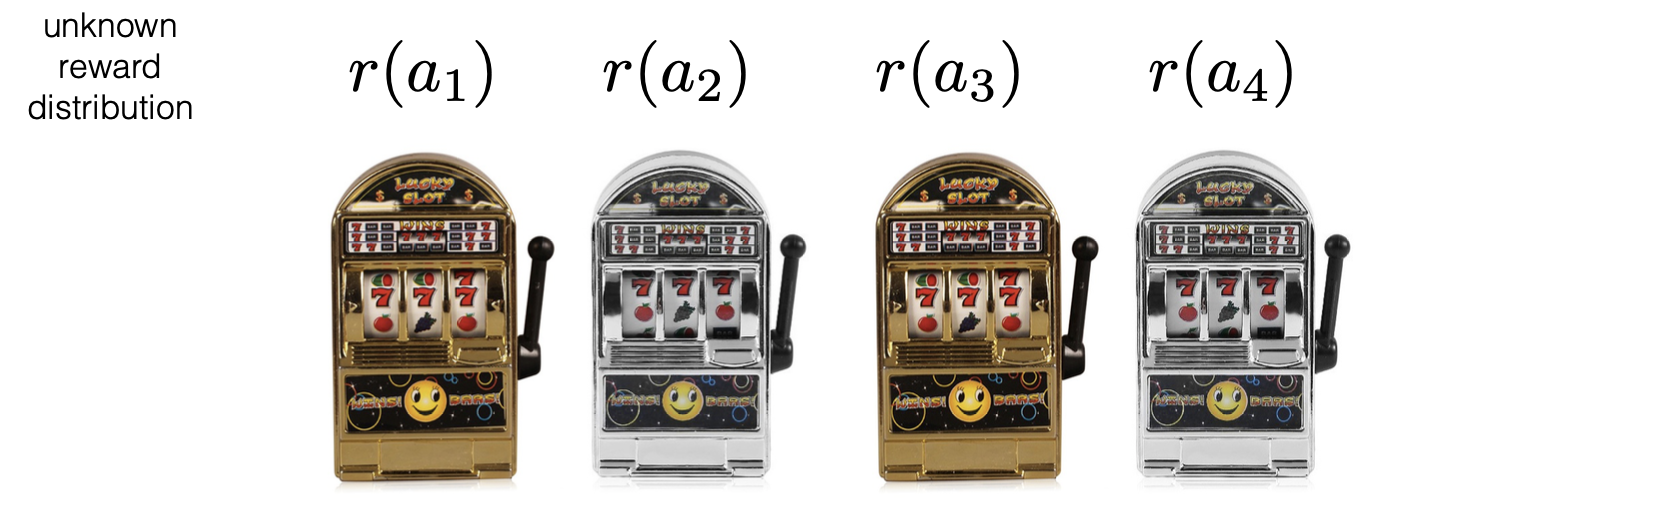
\includegraphics[width=0.8\textwidth]{figs/bandits.png}
    \caption{Multi-Armed Bandits.}
\end{figure}


Multi-armed bandits have the following characteristics:
\begin{enumerate}
    \item \textbf{One-Shot Feedback}: One action from the player leads to one reward and selecting any particular action does not change the state at the next time-step. 
    \item \textbf{Exhaustive Feedback}: The player can pull all the arms for the duration of the game, therefore actions are finite. The state is static and finite.
    \item \textbf{Evaluative Feedback}: The player receives a reward sampled from the underlying unknown reward distributions at each time-step.
\end{enumerate}
The goal of multi-armed bandit algorithms is to maximize the total reward the player over a horizon. Some applications of the MAB problem include:
\begin{enumerate}
    \item Advertisement Placement: Choosing which advertisement to display by giving reward if user clicks on the ad.
    \item Robotic Grasps: Choosing how to pick object where robot is rewarded if it graps an object.
\end{enumerate}

There is a tradeoff between exploration and exploitation in MAB problems.
We need to find a balance between exploiting arms that did well in the past vs exploring arms that might do well in the future. 

% There are different kinds of bandits based on the environment and number of states.

% \begin{figure}[H]
%     \centering
%     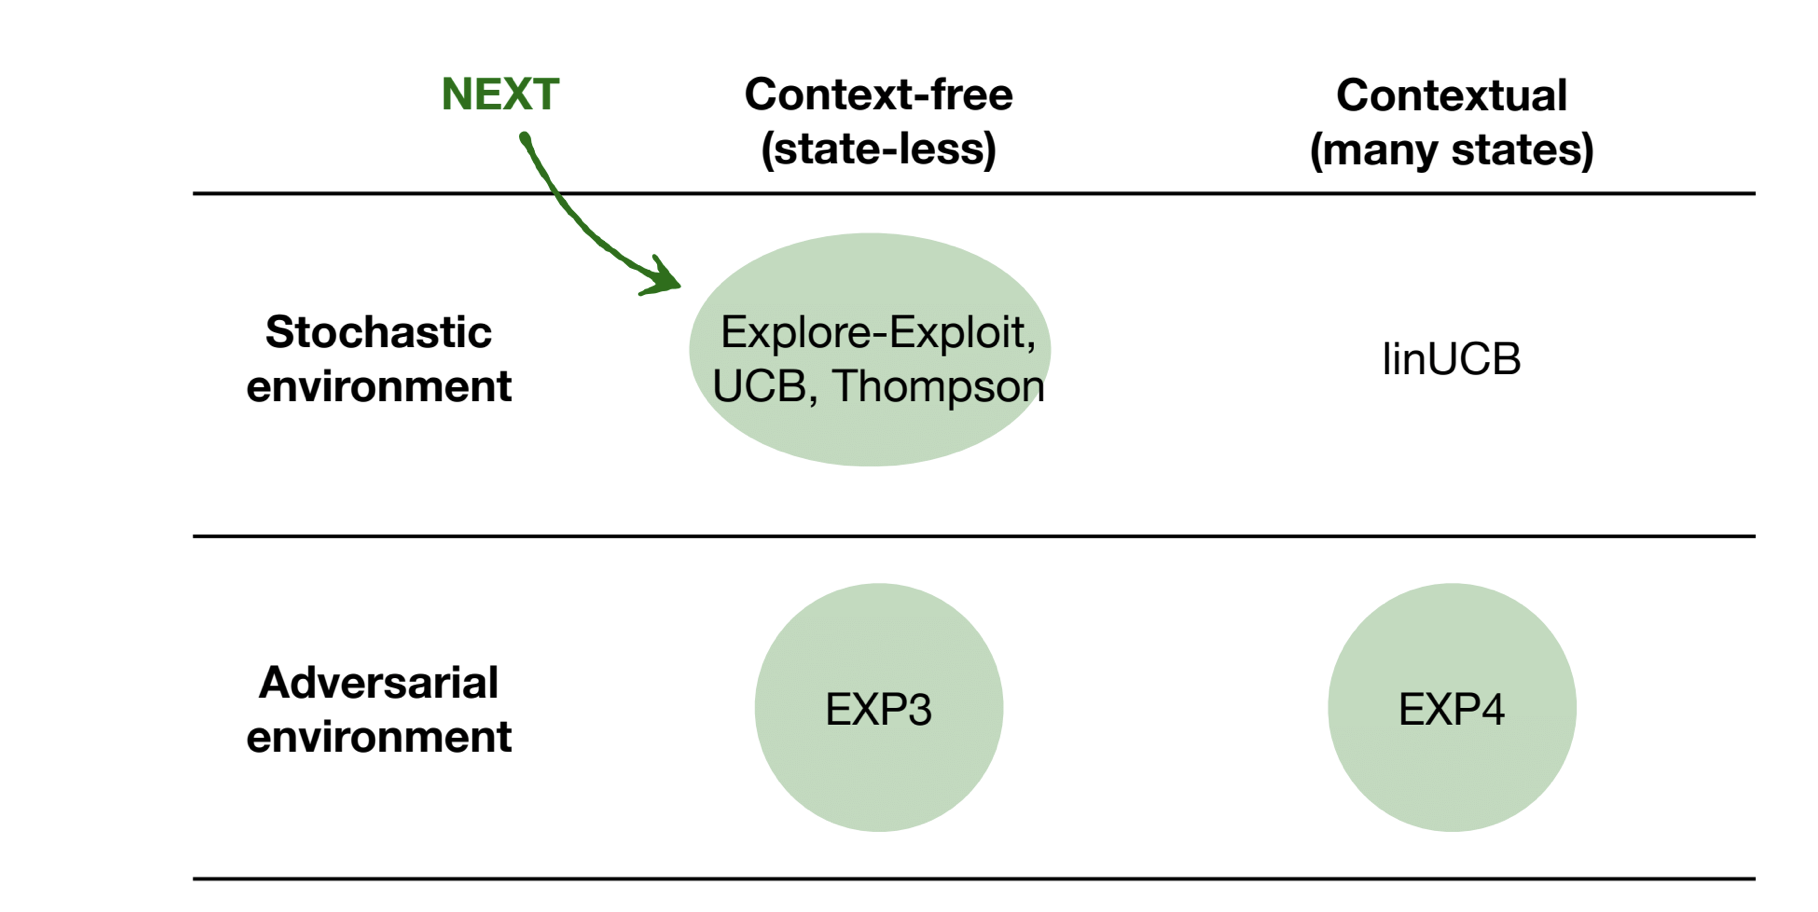
\includegraphics[width=0.8\textwidth]{figs/Screen Shot 2022-03-03 at 9.39.43 PM.png}
%     \caption{Types of Bandits.}
% \end{figure}

%This section serves as a review of the previous lecture and any other context required to frame the content of the current lecture. 

%You may format the scribes in any way you like, aside from changing font style, size and page format. Please use subsections and paragraphs to increase the readability of your notes.

%Length requirement 1-2 pages.

%TODO: INCLUDE TYPES OF BANDITS

\section{Summary}

In this lecture, we deal with stochastic (not adversarial) bandits. This essentially means that each bandit arm has a static reward distribution that does not change. Each arm pull essentially gives us a sample from the distribution. We saw in the previous lecture that given an estimated mean and the number of times an arm is pulled, it is not easy to say whether that arm is the most optimal arm for reward maximisation. 
% CHANGE THE FIGURE
\begin{figure}[h!]
    \centering
    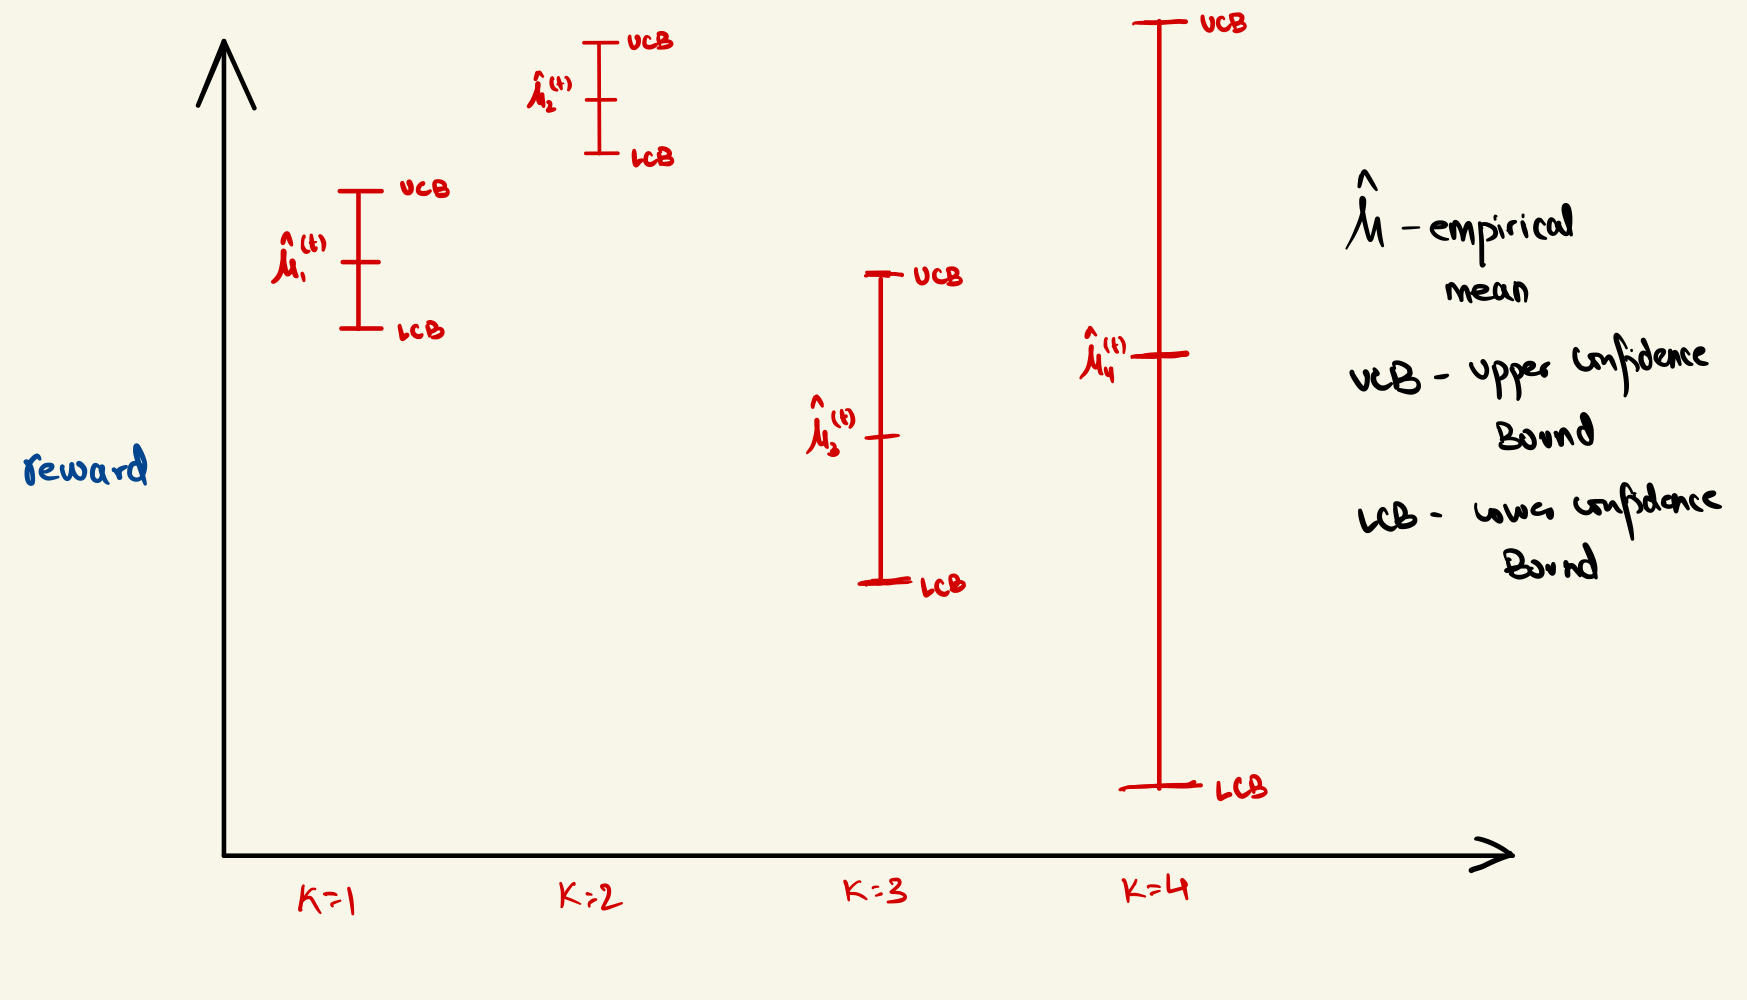
\includegraphics[width=0.8\textwidth]{IMG_0A1362EF257A-1.jpeg}
    \caption{Exploration vs Exploitation}
    \label{plot}
\end{figure}

%TODO ADD FIGURE

In Fig. \ref{plot}, a more conservative player would pick arm $k=2$ as $\hat{\mu}_{2}$ is the highest among other estimated mean values. Furthermore, the confidence bounds are also tight. On the other hand, a "gambler" would prefer high reward-high risk and choose the arm $k=4$. The conservative player is analogous to \textit{exploitation} and the gambler is analogous to \textit{exploration}.

\subsection{Explore-exploit algorithm}
Each Multi-arm bandit aims at reward maximisation by exploring or/and exploiting at each timestep.
This algorithm has two different stages. 
\begin{enumerate}
    \item \textbf{Explore Phase}: Pull each arm $M$ times to estimate the mean reward.
    \item \textbf{Exploit Phase}: Keep pulling the arm with the highest expected mean reward until $T$.
\end{enumerate}

\subsection{Multi-Armed Bandit: Explore-Exploit}
Algorithm. \ref{algo:explore-exploit} describes the Explore-Exploit algorithm.
\begin{algorithm}
\caption{Explore-Exploit}
\label{algo:explore-exploit}
\begin{algorithmic}[1]
\FOR{$k=1 \rightarrow K$}
\FOR{$m=1 \rightarrow M$}
\STATE $a = k$
\STATE $\mathtt{Receive}(r)$
\STATE $\hat{\mu}_k = \hat{\mu}_k + \frac{r}{M}$
\ENDFOR
\ENDFOR
\FOR{$t = KM \rightarrow T$}
\STATE $a^{(t)} = \arg \max_{k'} \hat{\mu}_{k'}$
\STATE $\mathtt{Receive}(r^{(t)})$
\ENDFOR
\end{algorithmic}
\end{algorithm}

Here, $K$ denotes the number of bandits, $M$ is the number of exploration steps per arm, and $T$ denotes the number of timesteps. Note that unlike online algorithms, $T$ here do not go to $\infty$. 

As we can see, this algorithm has two different stages. The first loop corresponds to the exploration stage where each arm is pulled $M$ times to estimate the mean $\hat{\mu} $ iteratively. The second loop employs exploitation. The algorithm picks the arm with the "best" estimated mean for the rest of the timesteps.


\subsubsection{Regret Analysis}

We will now derive the regret bound of the explore-exploit algorithm. However, before that, we need to discuss \normalfont \textbf{Hoeffding's Inequality} as it'll be used to derive the bounds.


%Note that the Hoeffding's Inequality can also be written as
%\[
%p \left( \left| \sum_{t=1}^T \frac{r^{(t)}}{T} - \mu \right| < \epsilon \right) %\geq 1 - 2 e^{-2T\epsilon^2}
%\]

% \begin{figure}
%     \centering
%     \includegraphics[width=0.5\textwidth]{images/ucb_lcb.png}
%     \caption{Illustrations of the definitions for the Lower Confidence Bound (LCB) and Upper Confidence Bound (UCB).}
%     \label{fig:ucb_lcb}
% \end{figure}


\theorem{\normalfont \textbf{Hoeffding's Inequality} Consider a one-dimension distribution $\nu$ with expectation
$\mu$, where any sample $r \sim \nu$ is bounded such that $r \in [0, 1]$. Given $T$ i.i.d samples, $\{ r^{(t)} \}_{t=1}^T$, we have that for any $\epsilon$: $$p \left( \left| \sum_{t=1}^T \frac{r^{(t)}}{T} - \mu \right| \geq \epsilon \right) \leq 2 e^{-2T\epsilon^2}$$ }


\normalfont

From the equation, we see that as we increase $T$, the probability that the absolute difference between estimated mean and actual mean would be greater than a given threshold decreases. In other words, this inequality means that the estimate of the mean gets better with the more samples are available. 

% We can also rewrite Hoeffding's Inequality as  :

% $$p \left( \left| \sum_{t=1}^T \frac{r^{(t)}}{T} - \mu \right| < \epsilon \right) \leq 1 - 2 e^{-2T\epsilon^2}$$



Say, we want the probability to be less than a given specified value $\delta$. In that case, we can then plug in $\delta$ into the inequality and solve for $\epsilon$:

\begin{align*}
    \delta = 2 e^{-2T\epsilon^2} \\
    log(\delta) = log(2) - 2T\epsilon^2 \\
     2T\epsilon^2 = log(2) - log(\delta) \\
     2T\epsilon^2 = log(\dfrac{2}{\delta}) \\
     \epsilon^2 = \dfrac{log(\dfrac{2}{\delta})}{2T} \\
     \epsilon = \sqrt{\dfrac{log(\dfrac{2}{\delta})}{2T}} \\
\end{align*}

This threshold, $\epsilon$, is called ``confidence interval" or ``confidence bound", as illustrated in Fig.~\ref{fig:confid}.
\begin{figure}[h!]
    \centering
    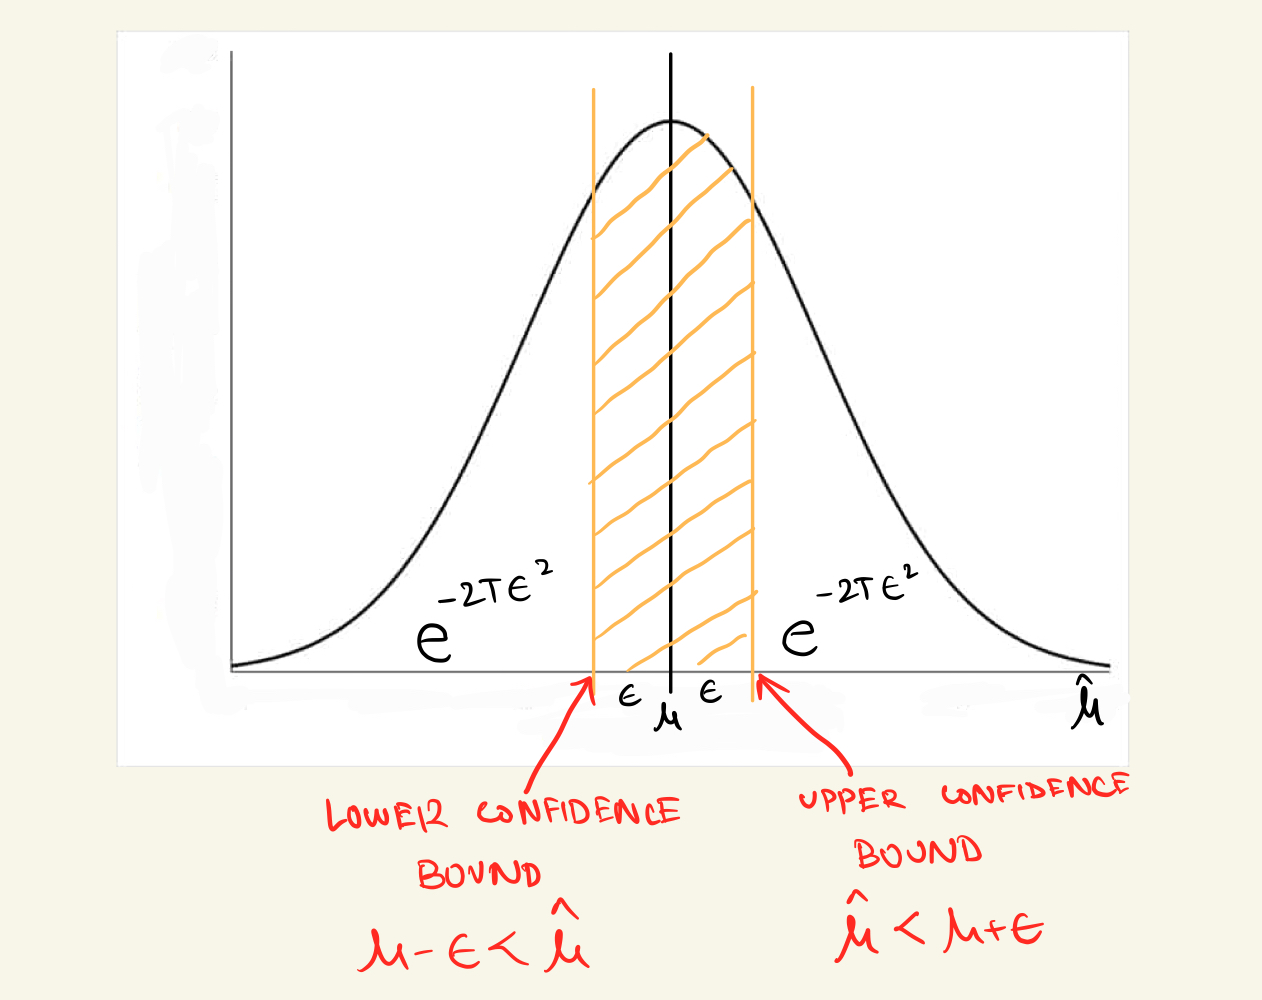
\includegraphics[width=0.5\textwidth]{IMG_3F1CB3131325-1.jpeg}
    \caption{An illustration of confidence interval.}
    \label{fig:confid}
\end{figure}

%TODO PROOF

Now, we can derive the regret bound for the Explore-Exploit algorithm. We divide the derivation in two steps: first for the exploration phase
and then for the exploitation phase.

\paragraph{Exploration Phase}
For the exploration phase, the worst case is that the algorithm gets no reward at any timestep. Say, the $k$th arm is the true best arm. For $M(K-1)$ steps the algorithm does not pick the best arm and therefore, there is a positive regret. In the exploration stage, when the algorithm pulls the $k$th arm, there could be a scenario where the rewards for those timesteps is not the best since rewards come from a stochastic distribution. Therefore, in worse case scenario, the regret bound for the exploration phase is $\mathcal{O}(KM)$.

$$ R_{\text{explore}} \leq \mathcal{O}(KM)$$

\paragraph{Exploitation Phase}
For the exploitation phase, we follow the five step procedure for finding bounds which is:
\begin{enumerate}
    \item Define the potential function.
    \item Upper bound the potential.
    \item Lower bound the potential.
    \item Combine the bounds.
    \item Use algebra to compute the regret bound.
\end{enumerate}
% EXPLAIN WHY THE INEQUALITY IS USED DIFFERENTLY
We first define the potential function using the fact
that if we pulled the wrong arm (i.e. not the true best arm), that means
our estimate of the best arm was wrong. Formally, our potential is defined
as
\[
\hat{\mu}_{\hat{k}} \geq \hat{\mu}_{k^*}
\] 
where $\widehat{k} = \arg\max_{k} \widehat{\mu}_k $ and $k^{\ast} = \arg\max_{k} \mu_k$. 

Notice that unlike prior algorithms, here we use an inequality as our potential function. Moreover, for computing the bounds of this potential function, we will essentially find the upper bound of $\hat{\mu}_{\hat{k}}$ and lower bound of $\hat{\mu}_{k^*}$. In other words, the least possible value of $\hat{\mu}_{\hat{k}}$ should still be higher than the greatest possible value of $\hat{\mu}_{k^*}$.

Now, we derive the upper and lower bounds as discussed above.

\textbf{Upper Bound} For the upper bound, we can use the Upper Confidence Bound (UCB) (derived using Hoeffding's Inequality) (illustrated
in Fig. \ref{fig:confid}):
\begin{align*}
\hat{\mu}_{\hat{k}} &\leq \mu_{\hat{k}} + \epsilon\\
&\leq \mu_{\hat{k}} + \sqrt{\frac{\log{2/\delta}}{2M}}
\end{align*}

\textbf{Lower Bound} For the lower bound, we can use the Lower Confidence Bound (LCB) (derived using Hoeffding's Inequality) (illustrated
in Fig. \ref{fig:confid}):
\begin{align*}
\hat{\mu}_{{k^*}} &\geq \mu_{k^*} - \epsilon\\
&\geq \mu_{k^*} - \sqrt{\frac{\log{2/\delta}}{2M}}
\end{align*}

% INEQUALITY USED HOW
\textbf{Combining Lower and Upper Bounds} We can combine these bounds 
\begin{align*}
\mu_{\hat{k}} + \sqrt{\frac{\log (2/\delta)}{2M}} &\geq \mu_{k^*} - \sqrt{\frac{\log (2/\delta)}{2M}}\\
\mu_{k^*} - \mu_{\hat{k}} &\leq 2 \sqrt{\frac{\log (2/\delta)}{2M}}\\
\end{align*}
The above equation shows the regret bound for one time step. We need to estimate the regret bound for all the timesteps (in the exploitation phase).
\begin{align*}
R_{\text{exploit}} &= \sum_{t=KM+1}^T (\mu_{k^*}^{(t)} - \mu_{\hat{k}}^{(t)}) \leq (T - KM) \cdot 2 \sqrt{\frac{\log (2/\delta)}{2M}}
\end{align*}

\paragraph{Combining Exploration and Exploitation Bounds}
We now have expressions for the regret bounds for the explore and exploit phases. We sum them to find the final expression for the regret of the explore-exploit algorithm.

\begin{align*}
    R_{\text{exploit}} &= (T-MK)(\mu_{k^{\ast}} - \mu_{\widehat{k}})\\
    &\leq (T-MK)2\sqrt{\frac{\log(2/\delta)}{2M}}\\
    &\leq \mathcal{O}\left(2(T-MK) \sqrt{\frac{1}{M}}\right).
\end{align*}

\begin{align*}
R_{\text{explore}} = \mathcal{O}(KM).
\end{align*}

\begin{align*}
    R &= R_{\text{explore}} + R_{\text{exploit}} \\
    &\leq \mathcal{O}(KM) +  \mathcal{O}\left(2(T-MK) \sqrt{\frac{1}{M}}\right)\\
    &\leq \mathcal{O}\left(KM + 2T \cdot \sqrt{\frac{1}{M}}\right)
\end{align*}

We see that the regret is linear in $T$, which would mean that the algorithm does not have a no-regret bound. If we want our
algorithm to be no-regret, we want the regret to grow sub-linearly. So, we can choose
$M$ in a way to make the regret sub-linear. We take the derivative of RHS and set it to zero.
\begin{align*}
    0 &= \frac{d}{dM} \Big\{ KM + 2T \cdot \sqrt{\frac{1}{M}} \Big\}\\
    0 &= K - TM^{-3/2}\\
    M &= \left( \frac{T}{K} \right)^{2/3}\\
\end{align*}

Note that, we need to know the total number of pulls $T$ in advance to get the optimal value of $M$. Plugging this optimal $M$ into our regret bound expression, we get:
\begin{align*}
    R &= R_{\text{explore}} + R_{\text{exploit}}\\
    &\leq KM + 2T \cdot \sqrt{\frac{1}{M}}\\ 
    &= K \left( \frac{T}{K} \right)^{2/3} + 2T \sqrt{\left( \frac{T}{K}\right)^{-2/3}}\\
    &= K \left( \frac{T}{K} \right)^{2/3} + 2T \left( \frac{T}{K}\right)^{-1/3}\\
    &= K^{1/3}T^{2/3} + 2T^{2/3}K^{1/3}\\
    &= 3K^{1/3}T^{2/3}\\
    &= \mathcal{O}(K^{1/3}T^{2/3})
\end{align*}

Thus, the regret bound for the Explore-Exploit algorithm is $R = \mathcal{O}(K^{1/3}T^{2/3})$. Note that this
is a sub-linear regret bound and that the total number of pulls $T$ is assumed to be known.

\subsection{Multi-Armed Bandit: Upper Confidence Bound}

Even though the explore-exploit algorithm is sublinear in time, it is not the best method and we can obtain lower regret bounds. Now, we discuss another algorithm called the Upper Confidence Bound (UCB) to solve a context-free bandit problem. UCB is an optimistic learner where the arm $k(t)$ with the largest mean reward ($\hat{\mu}_{k}$) plus a confidence term is picked. The algorithm is detailed in Algorithm.~\ref{algo:ucb}.

\begin{algorithm}[H]
\caption{Upper Confidence Bound (UCB) }
\label{algo:ucb}
\begin{algorithmic}[1]
\STATE Input: Time horizon $T$, Threshold $\delta'$
\FOR{$t=1 \rightarrow T$}
\IF{$t \le K$}
\STATE $k = t$ \hfill $\triangleright$ Initially pull each arm once (exploration)
\ELSE
\STATE $k = \argmax_{k'} \left(\hat{\mu}_{k'
} + \sqrt{\frac{\log(2T/\delta')}{2T_{k'}^{(t)}}} \right)$ \hfill $\triangleright$ mean reward + upper confidence
\ENDIF
\STATE $\mathtt{RECEIVE}(r^)$
\STATE $T_k^{(t)} = T_k^{(t)} + 1$  \hfill $\triangleright$ update pull counter for kth arm
\STATE $\hat{\mu}_{k} = \frac{1}{T_k^{(t)}}\left(\hat{\mu}_{k}(T_k^{(t)} - 1) + r^{(t)}\right)$ \hfill $\triangleright$ update mean reward for k
\ENDFOR
\end{algorithmic}
\end{algorithm}

\subsubsection{Understanding confidence term}
The confidence term is obtained using Hoeffding's inequality and depends on the number of pulls of a particular arm till time $t$ ($T_{k}^{(t)}$), total pulls ($T$) and threshold ($\delta$). So, as the game progresses and the number of pulls increase, the learner becomes more confident and the confidence term reduces.

\theorem{\normalfont\textbf{Boole's inequality (Union Bound)} The probability that at least one of the events happens is no
greater than the sum of the probabilities of the individual events. Mathematically, $p(\bigcup_i x_i) \le \sum_i p(x_i)$, where $x_i$'s are events.}\\


\normalfont\textbf{Proof Sketch} For two events $x_1$ and $x_2$, 
\begin{align*}
    p(x_1 \cup x_2) = p(x_1) + p(x_2) - p(x_1 \cap x_2)\\
p(x_1 \cup x_2) \le p(x_1) + p(x_2)\\
\end{align*}
The same logic can be extended to arbitary $n$ events. Using Hoeffding inequality (Theorem 1) and Union bound (Theorem 2), we get the confidence interval as:

\begin{align*}
    \mathbb{P}\left( \bigcup_{t=1}^{T} |\widehat{\mu}_k^{(t)} - \mu_k| > \sqrt{\frac{\log(2/\delta)}{2T^{(t)}_k}} \right) &\leq \sum_{t=1}^T \mathbb{P}\left(  |\widehat{\mu}_k^{(t)} - \mu_k| > \sqrt{\frac{\log(2/\delta)}{2T^{(t)}_k}} \right)\\
    &\leq T\delta.
\end{align*}
Then let $\delta' \triangleq T\delta$ we get 
\begin{equation}
    \epsilon' = \sqrt{\frac{\log(2T/\delta')}{2T^{(t)}_k}}.
\label{union_heoff}
\end{equation}

We will use the above theorem to derive the regret bound for UCB algorithm:.


\subsubsection{Regret Bound}
We will use the first five steps to calculate the regret bound starting from the potential function.

% % \theorem{\normalfont\textbf{Re}

The basic inequality that is defined is as follows, the learner may or may not select a non-optimal arm, until the confidence bound of the optimal arm is higher than that of the non-optimal arm. Mathematically, $k^*$ refers to the actual optimal arm, and $k^{(t)}$ refers to the estimated optimal arm at time step $t$:
$$\hat{\mu}_k^{(t)} + \sqrt{\frac{\log(2T/\delta')}{2T_{k}^{(t)}}} \ge \hat{\mu}_{k^*}^{(t)} + \sqrt{\frac{\log(2T/\delta')}{2T_{k^*}^{(t)}}}$$

We see the confidence bound in the inequality as it is also used to estimate the "best" arm at $t$ time step. s

\textbf{Upper Bound} We wish to obtain a upper bound on the predicted arm. From Hoeffding's inequality, we know that \begin{align*}
    |\hat{\mu}^{(t)} - \mu^{(t)}| \le \epsilon' \\
\end{align*}  
Using this, we have: 
$$\hat{\mu}_k^{(t)} \le \mu_k + \sqrt{\frac{\log(2T/\delta')}{2T_{k}^{(t)}}}$$
$$\mu_k + 2\sqrt{\frac{\log(2T/\delta')}{2T_{k}^{(t)}}} \ge \hat{\mu}_k^{(t)} + \sqrt{\frac{\log(2T/\delta')}{2T_{k}^{(t)}}}$$

\textbf{Lower Bound} We wish to obtain a upper bound on the arm from the base inequality that we derived. From Hoeffding's inequality, we know that 
\begin{align*}
    |\hat{\mu}^{(t)} - \mu | \le \epsilon' \\
\end{align*}
And we know that at time t,
$$\hat{\mu}_{k^*}^{(t)} \ge \mu_{k^*} - \sqrt{\frac{\log(2T/\delta')}{2T_{k^*}^{(t)}}}$$
$$\hat{\mu}_{k^*}^{(t)} + \sqrt{\frac{\log(2T/\delta')}{2T_{k^*}^{(t)}}} \ge \mu_{k^*} - \sqrt{\frac{\log(2T/\delta')}{2T_{k^*}^{(t)}}} + \sqrt{\frac{\log(2T/\delta')}{2T_{k^*}^{(t)}}}$$
$$\hat{\mu}_{k^*}^{(t)} + \sqrt{\frac{\log(2T/\delta')}{2T_{k^*}^{(t)}}} \ge \mu_{k^*}$$
\textbf{Combining the Upper and Lower Bounds} 
The lower bound is-
\begin{align*}
   \hat{\mu}_{k^*}^{(t)} + \sqrt{\frac{\log(2T/\delta')}{2T_{k^*}^{(t)}}} \ge \mu_{k^*}\\
    % \hat{\mu}_{k^*}^{(t)} - \mu_k \le 2\sqrt{\frac{\log(2T/\delta')}{2T_{k}^{(t)}}} \\
\end{align*}
And the upper bound as we defined is-
\begin{align*}
    \mu_k + 2\sqrt{\frac{\log(2T/\delta')}{2T_{k}^{(t)}}} \ge \hat{\mu}_k^{(t)} + \sqrt{\frac{\log(2T/\delta')}{2T_{k}^{(t)}}}
\end{align*}
Combining both the upper and lower bound, we get:
\begin{align*}
    \mu_k + 2\sqrt{\frac{\log(2T/\delta')}{2T_{k}^{(t)}}} \ge \mu_{k^*} \\
    \mu_{k^*} -  \mu_k \leq 2\sqrt{\frac{\log(2T/\delta')}{2T_{k}^{(t)}}}
\end{align*}
This being for one instance, if we are pulling an arm $k$ for each time instant $t$, then we have-
$$\mathcal{R}_{UCB} = \sum_{t=1}^T (\mu_{k^*} - \mu_{k^{(t)}})$$
$$ \leq \sum_{t=1}^T 2\sqrt{\frac{\log(2T/\delta')}{2T_{k^{(t)}}^{(t)}}}$$
$$ = 1/2\sqrt{\log(2T/\delta')} \sum_{t=1}^T 
\sqrt{\frac{1}{T_{k^{(t)}}^{(t)}}}$$
We do this process to factor out constants. Next, we change the notation using a sum over arms.
$$ = 1/2\sqrt{\log(2T/\delta')} \sum_{t=1}^T \sum_{j=1}^K \mathbbm{1}[k^{(t)} = j]\sqrt{\frac{1}{T_{j}^{(t)}}}$$
$$ = 1/2\sqrt{\log(2T/\delta')} \sum_{j=1}^K \sum_{t=1}^T \mathbbm{1}[k^{(t)} = j]\sqrt{\frac{1}{T_{j}^{(t)}}}$$
$$ = 1/2\sqrt{\log(2T/\delta')} \sum_{j=1}^K \sum_{t=1}^{T_j^{(T)}} \sqrt{\frac{1}{t}}$$

There are two mathematical inequalities required to derive the regret bound as discussed in the lecture, namely Jensens inequality and the summation bound-
\theorem{\normalfont\textbf{Jensen's Inequality} Iff $f$ is a convex function, $f(\sum_nP_nx_n) \le \sum_nP_nf(x_n)$. }

\fact{Summation Bound in the lecture slides:}
$$\sum_{t=1}^{T}\sqrt{\frac{1}{t}} \le 2\sqrt{T}$$
The proof is as follows
\begin{align*}
    \sum_{t=1}^{T}\sqrt{\frac{1}{t}} = 1 + \sum_{t=2}^{T}\sqrt{\frac{1}{t}} \\
    \le 1 + \int_{t=1}^{T} \sqrt{\frac{1}{t}}dt \\
    = 1 + 2 \sqrt(T) - 2 = 2 \sqrt{T} - 1 \\
    \le 2 \sqrt{T}
\end{align*}
\begin{figure}[h]
    \centering
    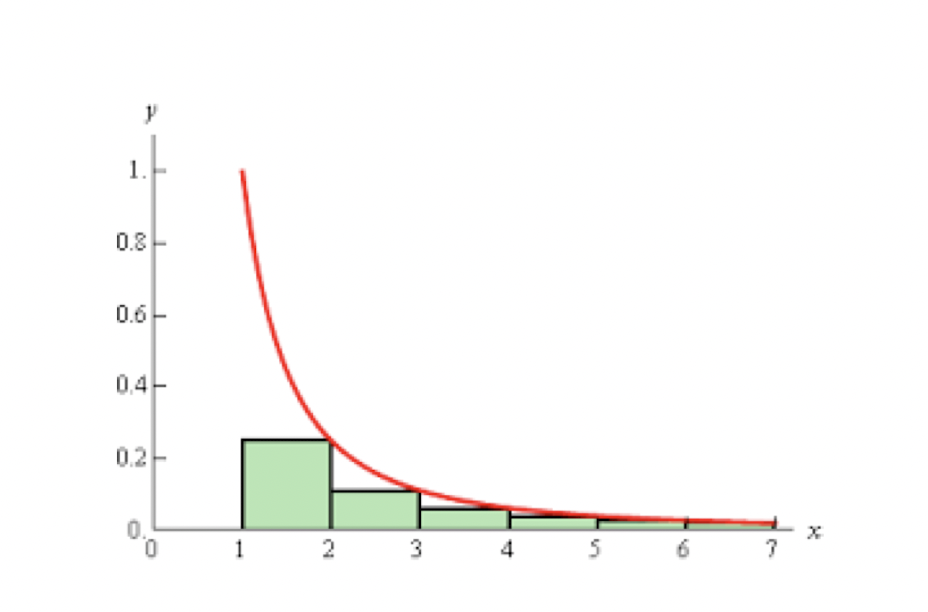
\includegraphics[scale=0.5]{figs/Screen Shot 2022-03-04 at 12.30.28 AM.png}
    \caption{Graphical form of the summation bound}
    \label{fig:my_label}
\end{figure}


\normalfont
Plugging in our equation
$$\mathcal{R}_{UCB} \le \sqrt{\log(2T/\delta')} \sum_{j=1}^K \sum_{t=1}^{T_j^{(T)}} \sqrt{\frac{1}{t}}$$
$$\le 1/2\sqrt{\log(2T/\delta')} \sum_{j=1}^K 2\sqrt{T_j^{(T)}} \qquad \text{(Using Summation bound )}$$
$$\le \sqrt{8\log(2T/\delta')} K \left(\frac{1}{K}\sum_{j=1}^K \sqrt{T_j^{(T)}} \right)$$
$$\le \sqrt{\log(2T/\delta')} K \left( \sqrt{\frac{1}{K}\sum_{j=1}^K T_j^{(T)}} \right)  \qquad \text{(Using Jensen's inequality)}$$
$$= \sqrt{\log(2T/\delta')} K \left( \sqrt{\frac{T}{K}} \right)$$
$$= \sqrt{\log(2T/\delta')} \sqrt{TK} \approx \mathcal{O}(\sqrt{TK})$$

If we compare, the regret bound for UCB ($\mathcal{O}(\sqrt{T}$) is "more" sub-linear with respect to $T$ than Explore-Exploit algorithm ($\mathcal{O}(T^{\frac{2}{3}})$) and hence, is better. If we dive further to understand this behaviour, we'll see that in UCB, the confidence bound of a "good" arm gets tighter with time.  This statement can be supported by looking at the equation computing confidence of an arm. We see that $T_{k'}^{(t)}$ is in the denominator, which denotes that as the number of times the arm is pulled increases, its confidence bounds gets tighter and the algorithm gets a better estimate of "good" arms. Next, the algorithm prefers "good" arms and furthermore results in tighter confidence bounds.
This behaviour correlates with exploiting rather than exploring.
\begin{equation*}
    \epsilon = \sqrt{\frac{\log(2T/\delta')}{2T_{k'}^{(t)}}}
\end{equation*}

Therefore, unlike explore-exploit which has fixed timesteps for exploring, UCB starts exploiting as the confidence bounds get tighter.


%\section*{References}
%Include your references here. Please cite any resources you found useful.	
%Populate the refs.bib file or list your references manually. Be consistent in formatting!
\newpage
{
\bibliography{refs}
\bibliographystyle{abbrv}
}

\section{Appendix}
The proof of the Hoeffdings inequality is as follows-
Let $Z_1, Z_2, .... Z_n$ be random bounded variables such that $Z_i \in [0,1]$ with probability 1. Hence Z is a random variable with $E[Z]=0$ and $0 \le Z \le 1$, then by Chernoff's bound[1], we have 
\begin{align*}
    E[e^{sZ}]\le e^{\frac{s^2}{8}}
\end{align*}
By the convexity of the exponential function, we have 
\begin{align*}
    e^{sZ} \le ze^s + (1-z)e^0, 0 \le z \le 1 \\
    E[e^{sZ}] \le E[Z]e^{s} + E[1-z]e^0 \\
    E[Z]=0 \\
    \text{Hence} \\
    E[e^{sZ}] \le 1
\end{align*}
If we say that $\phi$ is a function of s then, we can write this as
\begin{align*}
    E[e^{sZ}] \le e^{\phi(s)}
\end{align*}
To minimize the upper bound, let us express $\phi(s)$ as a taylor's series with a remainder-
\begin{align*}
    \phi(s) = \phi(0) + s \phi'(0) + \dfrac{s^2}{2}\phi''(v), v \in [0,s] \\
    \phi'(s)=0,  \phi''(s)\le 1/4\\
    \text{From this} \\
    \phi(s) \le s^2 /8 \\
    E[e^{sZ}] \le e^{s^2 /8}
\end{align*}
Applying this as an upper bound to derive Hoeffdings inequality- 
\begin{align*}
    P(S_n - E[S_n] \ge t) \le 2e^{-2T\epsilon^2} \\ 
    \text{In terms of the slide-} \\
    p \left( \left| \sum_{t=1}^T \frac{r^{(t)}}{T} - \mu \right| \geq \epsilon \right) \leq 2 e^{-2T\epsilon^2}
\end{align*}
\newpage
\section{References}
[1] https://nowak.ece.wisc.edu/SLT07/lecture7.pdf
%This section provides any relevant background material that was not covered in the lectures, but was found to be useful for understanding the material. 
%For example, derivations, theory underlying techniques employed, etc. 

%Additionally, this section can summarizes applications or extensions of these techniques found in the literature. 

\end{document} % Done!

